\section{显微镜}

显微镜分为光学显微镜、电子显微镜、扫描隧道显微镜三种。它们三者之间除了都能放大微观结构之外,没有任何共同之处。

\begin{figure}[htbp]
	\centering
	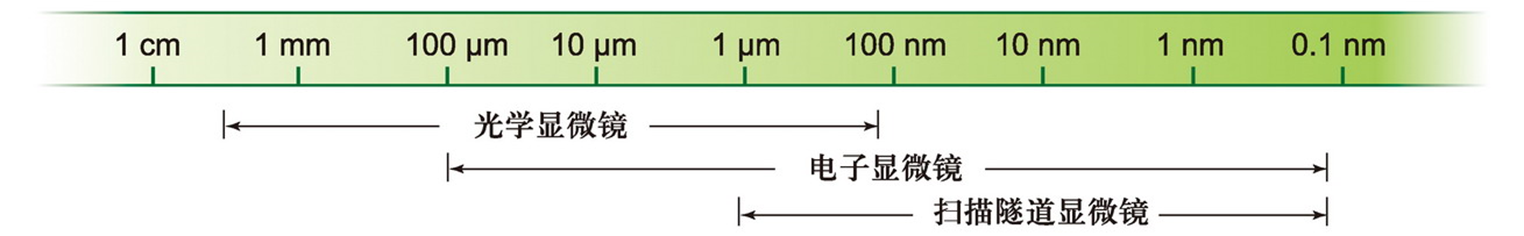
\includegraphics[width=\linewidth]{Pics/三种显微镜的分辨率范围}
	\caption{三种显微镜的分辨率范围}
	\label{fig:threeTypesOfMicroscopesResolutionRange}
\end{figure}


\subsection{光学显微镜}

\begin{figure}[htbp]
	\centering
	\begin{forest}
		forest scheme
		[光学显微镜
		[普通光学显微镜]
		[相差显微镜、微分干涉显微镜]
		[荧光显微镜]
		[激光扫描共聚焦显微镜]
		[超高分辨率显微术
		[TIRFM]
		[PALM/STORM]
		[4$\pi$]
		[STED]
		[SIM]]]
	\end{forest}
	\caption{光学显微镜技术的分类}
	\label{fig:opticalMicroscopyTechniquesClassification}
\end{figure}

\subsubsection{普通光学显微镜}

显微镜最重要的参数是分辨率,即能分辨出的距离最小的两点之间的距离。分辨率\[D=\frac{0.61\lambda}{N\cdot\sin\dfrac{\alpha}{2}}\]

其中;(\autoref{fig:opticalMicroscopeResolutionInfluencingFactors})
\begin{description}
	\item[$\lambda$] 光源的波长;
	\item[$N$] 介质折射率,空气为1,香柏油为1.5;
	\item[$\alpha$] 镜口角;
	\item[NA(数值口径,镜口率)] 全称是Numerical Aperture,即$N\cdot\sin\frac{\alpha}{2}$。
\end{description}

\begin{figure}[htbp]
	\centering
	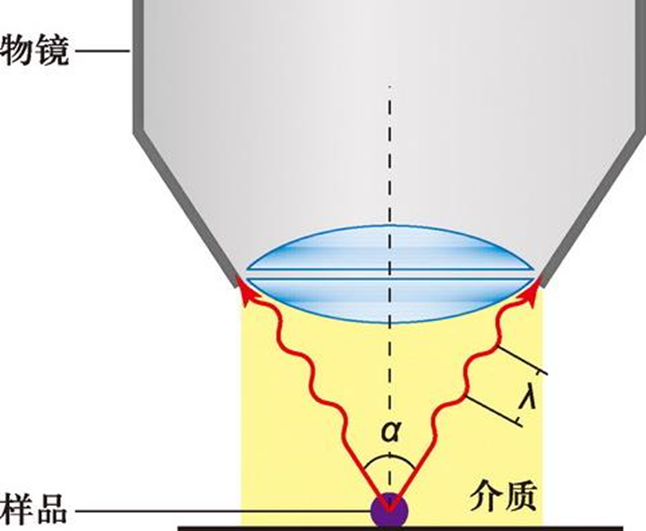
\includegraphics[width=0.4\linewidth]{Pics/光学显微镜的分辨率影响因素}
	\caption{光学显微镜的分辨率影响因素}
	\label{fig:opticalMicroscopeResolutionInfluencingFactors}
\end{figure}

光学显微镜达到最大分辨率时,以上参数分别为:
\begin{itemize}
	\item $\alpha=\SI{140}{\degree}$;
	\item 油镜下,$N=1.5$;
	\item 可见光波长最短为\SI{400}{\nm};
\end{itemize}

计算可得普通光学显微镜最大分辨率为\SI{0.2}{\um}。

\subsubsection{相差显微镜和微分干涉显微镜}

光线通过不同密度的材质时,会发生不同程度的“滞留”,密度大则滞留时间长,由此造成了光相位的差异。相位相反的光,振幅会被抵消至0,相位相同的光,振幅就相互叠加。(\autoref{fig:interferenceBetweenTwoLightBeams})由此,相差显微镜就把样品中密度的不同,转换为视野中图像亮度的差异。相差显微镜可以观察活细胞。

\begin{figure}[htbp]
	\centering
	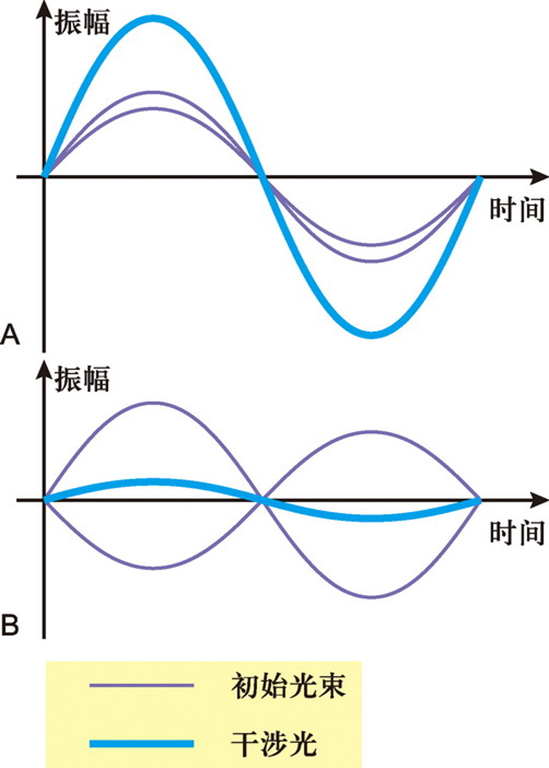
\includegraphics[width=0.4\linewidth]{Pics/两束光之间的相互干涉}
	\caption{两束光之间的相互干涉}
	\label{fig:interferenceBetweenTwoLightBeams}
\end{figure}

Nomarski在相差显微镜的基础上,改进出微分干涉显微镜。它以平面偏振光为光源,更适合研究活细胞。

将微分干涉显微镜接上录像装置,计算机辅助的微分干涉显微镜可以降低背景噪声、提高样品反差,大大提高了分辨率。应用这一原理制备的录像增差显微镜甚至可以直接观察微管参与的物质运输。

\subsubsection{暗视野显微镜}

聚光镜中央有挡光片,视野背景是黑的,只允许被标本反射和衍射的光线进入物镜,物体边缘是亮的。可观察4\textasciitilde\SI{200}{\um}的微粒子,分辨率比普通显微镜高50倍。(\autoref{fig:dkfld_mcscp})

\begin{figure}[htbp]
	\centering
	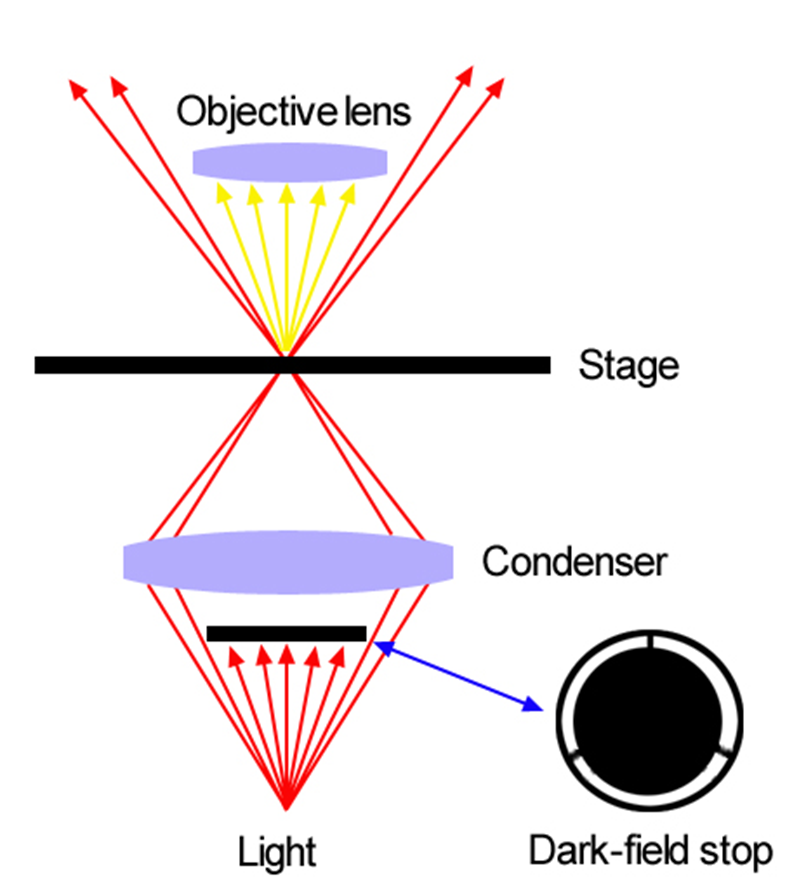
\includegraphics[width=0.4\linewidth]{Pics/暗视野显微镜}
	\caption{暗视野显微镜成像原理}
	\label{fig:dkfld_mcscp}
\end{figure}

在\autoref{fig:comparision_mcscp1}中,A图是普通光镜、B图是相差显微镜、C图是微分干涉显微镜、D图是暗视野显微镜所成的像。

\begin{figure}[htbp]
	\centering
	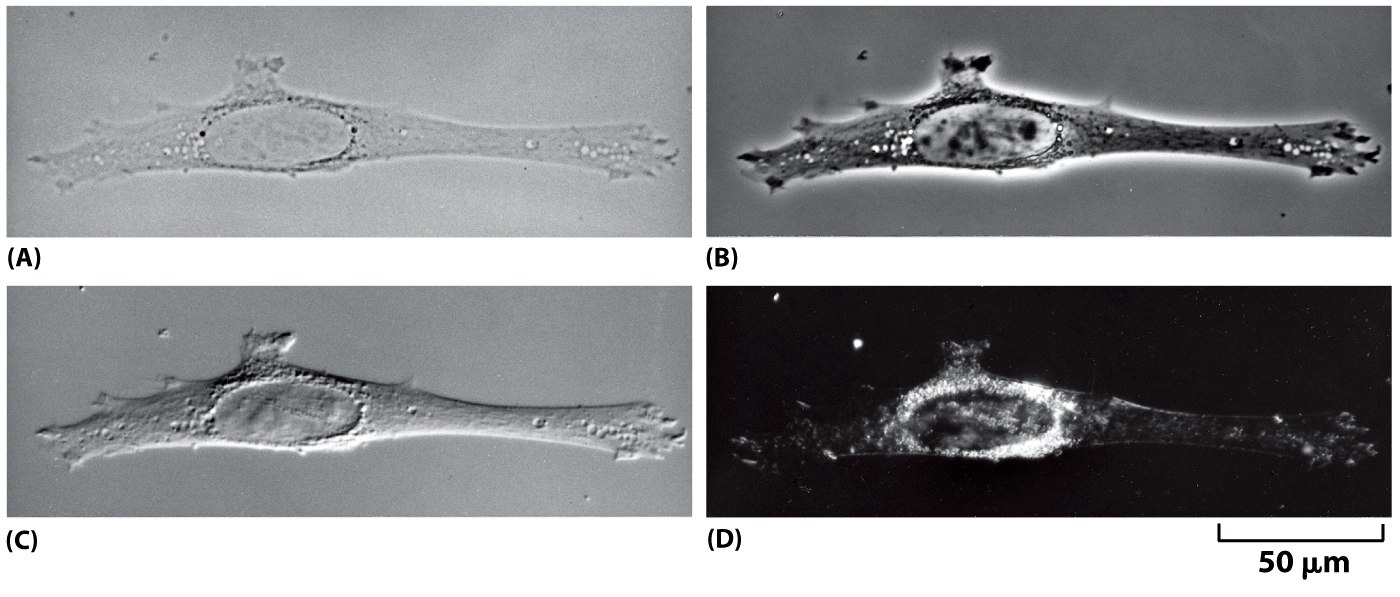
\includegraphics[width=0.8\linewidth]{Pics/显微镜成像对比}
	\caption{不同显微镜成像的对比}
	\label{fig:comparision_mcscp1}
\end{figure}

\subsubsection{荧光显微镜}

荧光显微镜的核心部件是滤光片系统和专用的物镜镜头。滤光片系统由激发滤光片和阻断滤光片组成。激发滤光片只允许特定波长的激发光通过,阻断滤光片只允许荧光染料所发出的荧光通过。(\autoref{fig:fluorescenceMicroscopeImagingPrinciple})

绿色荧光蛋白(GFP,\autoref{fig:gfp})是常用的荧光标记,只需将其与目标蛋白融合表达即可。

\begin{figure}[htbp]
	\centering
	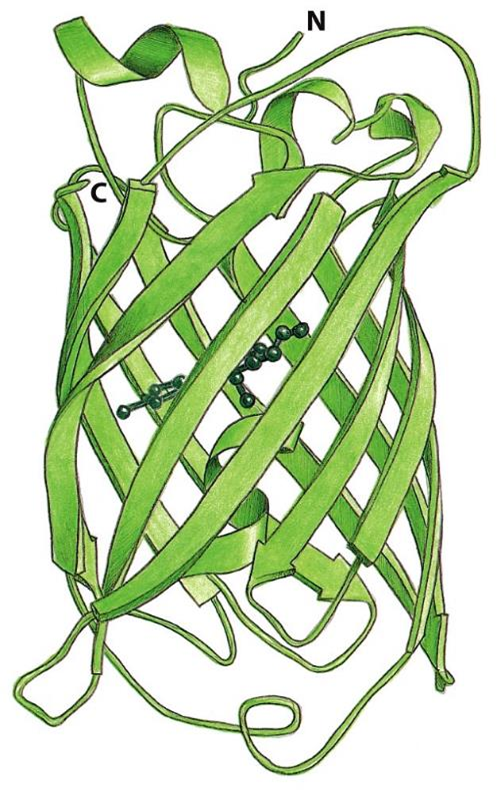
\includegraphics[width=0.3\textwidth]{Pics/GFP}
	\caption{绿色荧光蛋白的结构}
	\label{fig:gfp}
\end{figure}

\begin{gs}[:GFP与诺贝尔奖]

	\hspace{2em}马丁·查尔菲(Martin Chalfie)、钱永健、下村修(Osamu Shimomura)三人因发现GFP获得诺贝尔奖。

	\hspace{2em}道格拉斯·普瑞舍(Douglas C. Prasher)是一名美国的分子生物学家。因为他对荧光蛋白水母素 (aequorin)克隆和测序而广为科学界所知。他早年曾将他的科研经验与成果与钱永健和马丁·查尔菲 (Martin Chalfie)分享过,但是他自己却因为无法获得足够的实验经费而不得不离开学术界。最终,他完全放弃了科学工作。2008年查尔菲与钱永健因为他们对于GFP的贡献而获得诺贝尔化学奖,而他们的研究极大程度是基于普瑞舍当年的研究成果上。由于这两名诺贝尔奖得主的努力,普瑞舍终于在钱永健的资助下于2010年6月回归学术界,目前在钱永健的实验室工作。
\end{gs}

\begin{figure}[htbp]
	\centering
	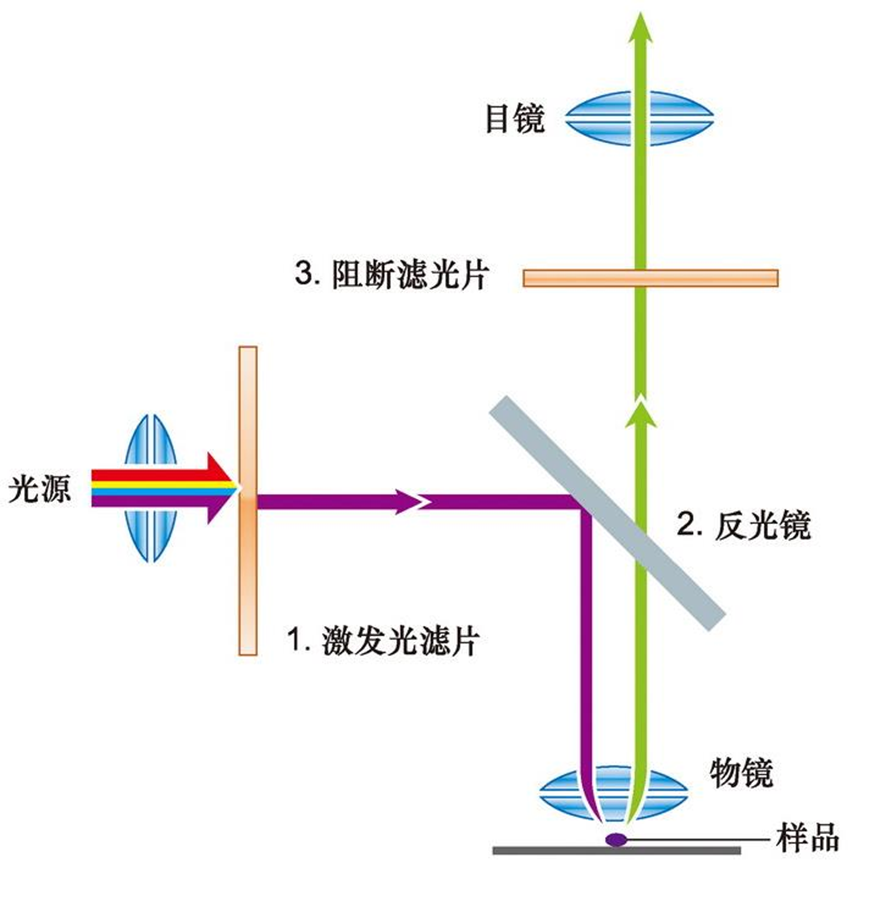
\includegraphics[width=0.4\linewidth]{Pics/荧光显微镜成像原理}
	\caption{荧光显微镜成像原理}
	\label{fig:fluorescenceMicroscopeImagingPrinciple}
\end{figure}

短波长的激发光通过激发滤光片,使样品中的荧光分子产生波长较长的荧光。荧光显微镜的暗视野提供了强反差背景,使微弱的荧光信号得以分辨。

\subsubsection{激光扫描共聚焦显微镜(LSCM)}

普通荧光显微镜下,来自不同焦平面的光线会互相干扰,导致图像模糊不清。激光扫描共聚焦显微镜相当于多安装了一套激光共焦成像系统,以激光或紫外光为光源,大大提高分辨率。共焦的意思就是,物镜和聚光镜的焦点在同一处。焦平面以外的光线就被遮挡住,因此只有来自焦平面的光线才可被观察。(\autoref{fig:LSCM},\autoref{fig:comparisonOfImagesObservedByFluorescenceMicroscopyAndLaserScanningConfocalMicroscopy})

由于观察到的画面只来自样品的一个焦平面,观察的焦平面还可以自动调整,故可以通过改变焦平面来进行“光学切片”,重构细胞的三维图像。

\begin{figure}[htbp]
	\centering
	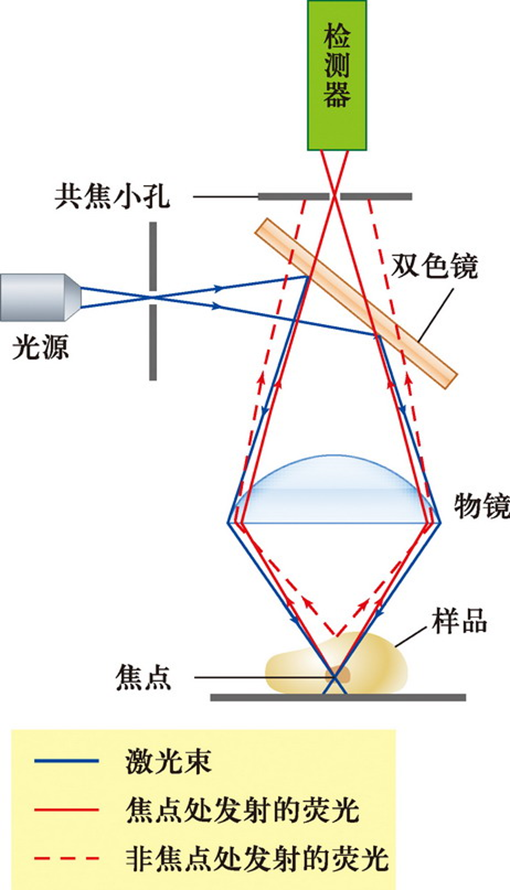
\includegraphics[width=0.3\textwidth]{Pics/激光扫描共聚焦显微镜}
	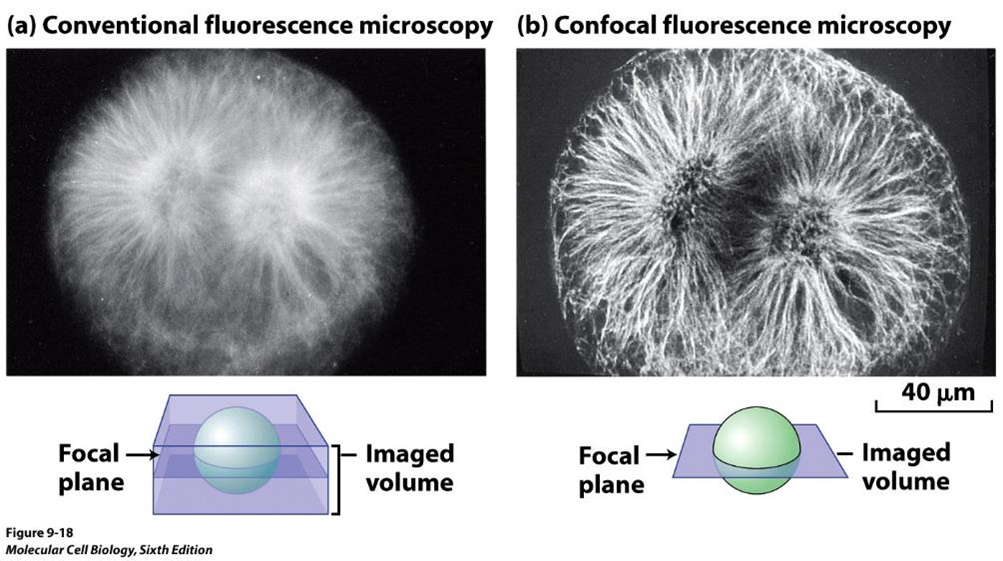
\includegraphics[width=0.5\textwidth]{Pics/激光扫描共聚焦显微镜2}
	\caption{激光扫描共聚焦显微镜成像原理}
	\label{fig:LSCM}
\end{figure}


\begin{figure}[htbp]
	\centering
	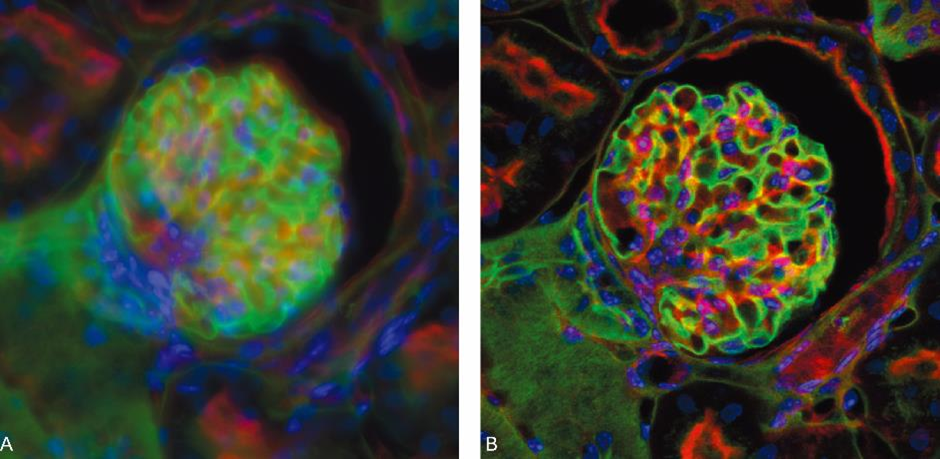
\includegraphics[width=0.7\linewidth]{Pics/荧光显微镜和激光扫描共焦显微镜所观察图像的比较}
	\caption{荧光显微镜(A)和激光扫描共焦显微镜(B)所观察图像的比较}
	\label{fig:comparisonOfImagesObservedByFluorescenceMicroscopyAndLaserScanningConfocalMicroscopy}
\end{figure}

\subsubsection{超高分辨率显微术}

\paragraph{全内反射荧光显微术(TIRFM)}

降低噪声是提高显微镜分辨率的有效途径。在LSCM中,已经通过小孔来阻挡非焦平面的光线,可是小孔不可以无限缩小。在TIRFM中,光线发生全反射时,在介质另一侧激发出的隐失波波长在\SI{200}{\nm}之内,而且衰减快,故可激发很薄一层样品内的荧光。该技术的特点是只能观细胞紧靠玻片约\SI{100}{\nm}的范围。(\autoref{fig:TIRFM})

\begin{figure}
	\centering
	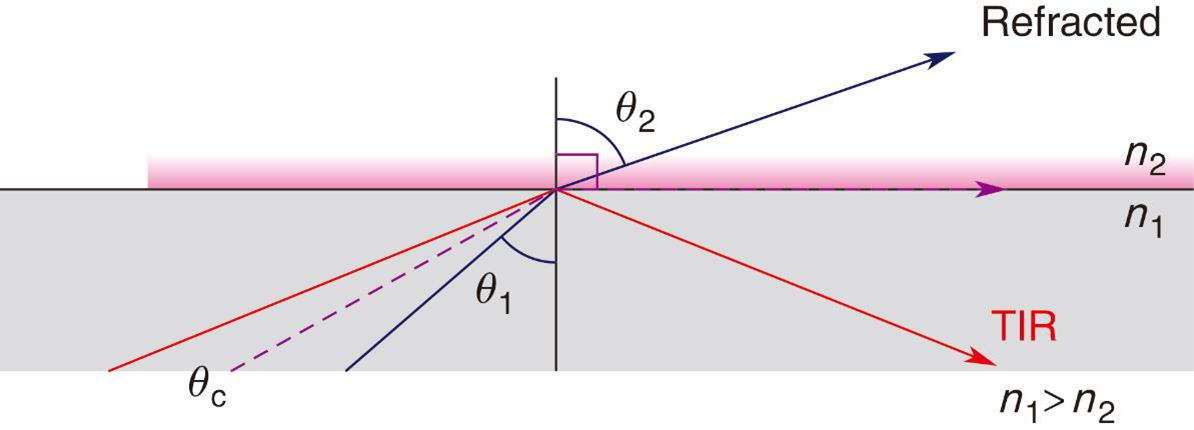
\includegraphics[width=0.7\linewidth]{Pics/TIMFR}
	\caption{TIRFM的原理}
	\label{fig:TIRFM}
\end{figure}


\paragraph{PALM/STORM}

见书本。

\paragraph{$4\pi$和STED显微术}

$4\pi$显微镜通过在样品的两侧各放置一个高性能物镜,使镜口角扩大到接近$4\pi$,从而提高了数值口径,有效提高了z轴分辨率。

但是,$4\pi$显微镜并没有突破衍射极限。在受激发射损耗(STED)显微术中,通过环状激光使一个点周围的荧光基团淬灭,只有中间那个点可以被观察到。理论上,只要减小环状激光中间的孔径,就可以实现纳米级别的分辨率。STED并没有提高z轴方向的分辨率。

\paragraph{结构照明显微术}

在显微镜中增加光栅和控制元件。优点是对于普通的样本,可以不经特殊处理直接观察。缺点是分辨率远低于其他超高分辨率显微术。

\subsection{电子显微镜}

\subsubsection{电子显微镜的基本知识}

\paragraph{与光镜的区别}

见\autoref{tab:comparisonBetweenOpticalMicroscopeAndElectronMicroscope}。

\begin{table}[htbp]
	\centering
	\begin{tabularx}{\textwidth}{|c|c|c|c|c|C|}
		\hline
		显微镜类型 & 分辨本领 & 光源 & 透镜 & 真空 & 成像原理 \\ \hline
		光学显微镜 & \SI{0.2}{\um} & 可见光 & 玻璃 & 无需 & 吸光形成明暗反差和颜色变化 \\ \hline
		电子显微镜 & \SI{0.2}{\nm} & 电子束 & 电磁 & 真空 & 电子散射和透射形成明暗反差 \\ \hline
	\end{tabularx}
	\caption{光学显微镜和电子显微镜的对比}
	\label{tab:comparisonBetweenOpticalMicroscopeAndElectronMicroscope}
\end{table}

\paragraph{电镜的分辨率}

电子显微镜的图像不可直接观察,要通过荧光屏、感光胶片或电荷耦合器件(CCD)来成像。

电镜的分辨率和分辨本领并不是一回事。分辨本领指的是最理想情况下的分辨率,也即最大分辨率。而实际的分辨率常常受到制样技术的限制,如超薄切片样品中,分辨率约为超薄切片厚度的$\frac{1}{10}$。

人眼的分辨率约为\SI{0.2}{\mm}。用人眼分辨率除以光镜和电镜的分辨率即可得到各自的放大倍数。所以,光镜的放大倍数约为1000,电镜的放大倍数约为$10^6$。

\paragraph{电子显微镜的构造}

较为原始的电子显微镜的结构如\autoref{fig:emstrctr}所示,但是其成像原理并没有和现代的电镜有很大不同。

\begin{figure}[htbp]
	\centering
	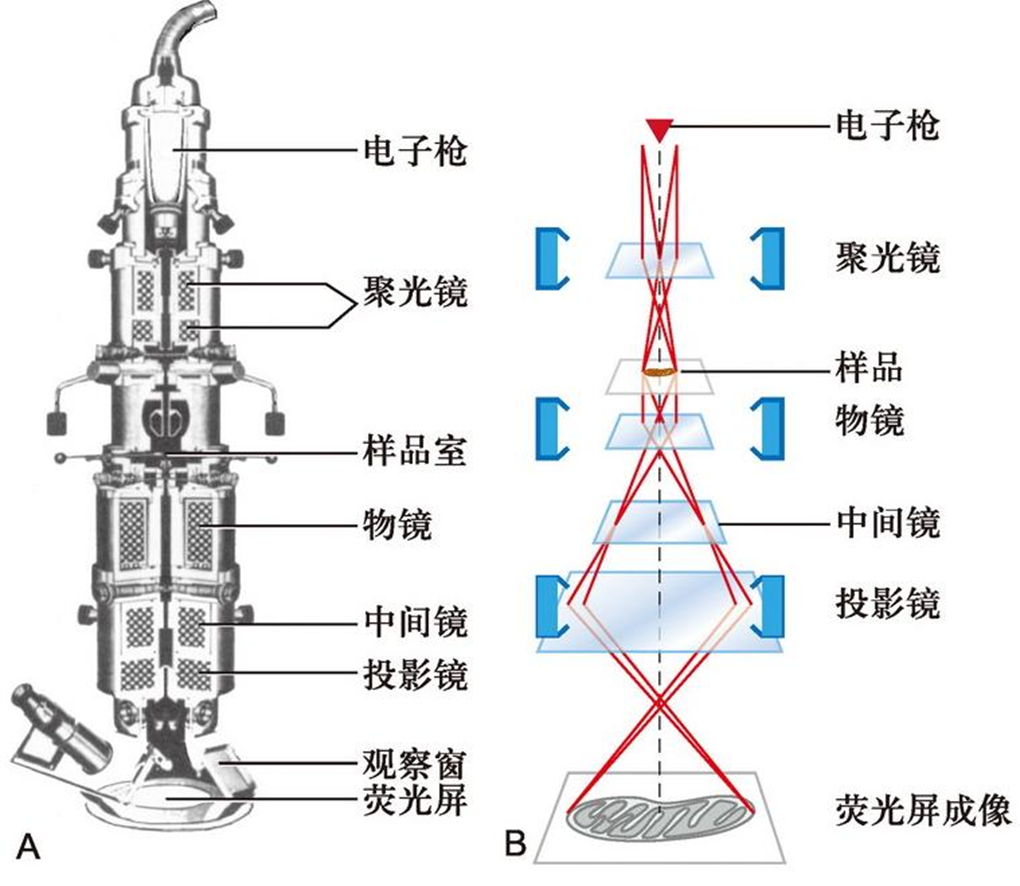
\includegraphics[width=0.5\linewidth]{Pics/EM_strctr}
	\caption{电子显微镜的结构}
	\label{fig:emstrctr}
\end{figure}

电子显微镜由以下4部分构成:
\begin{description}
	\item[电子束照明系统] 包括电子枪和聚光镜。例如,可加热钨丝发射电子,通过高电压的阳极加速电子。
	\item[成像系统] 物镜、中间镜、投影镜等精密中空圆柱体内有磁场,使电子聚焦。
	\item[真空系统] 真空泵不断抽气,保持镜筒内真空。
	\item[记录系统] 通过荧光屏、感光胶片或CCD记录。
\end{description}

\subsubsection{主要电镜制样技术}

\paragraph{超薄切片}

电子束穿透能力有限,为获得较高分辨率就要将切片变得薄,一个切片只有40\textasciitilde\SI{50}{\nm}厚。这要求样品具有一定的韧性和刚性,所以要对样品进行包埋。为了在包埋过程中尽可能保留细微结构,需要先对样品进行固定。操作流程为:固定$\longrightarrow$包埋$\longrightarrow$切片$\longrightarrow$染色。(\autoref{fig:prcs_ultr_thn_sctn})

\begin{figure}[htbp]
	\centering
	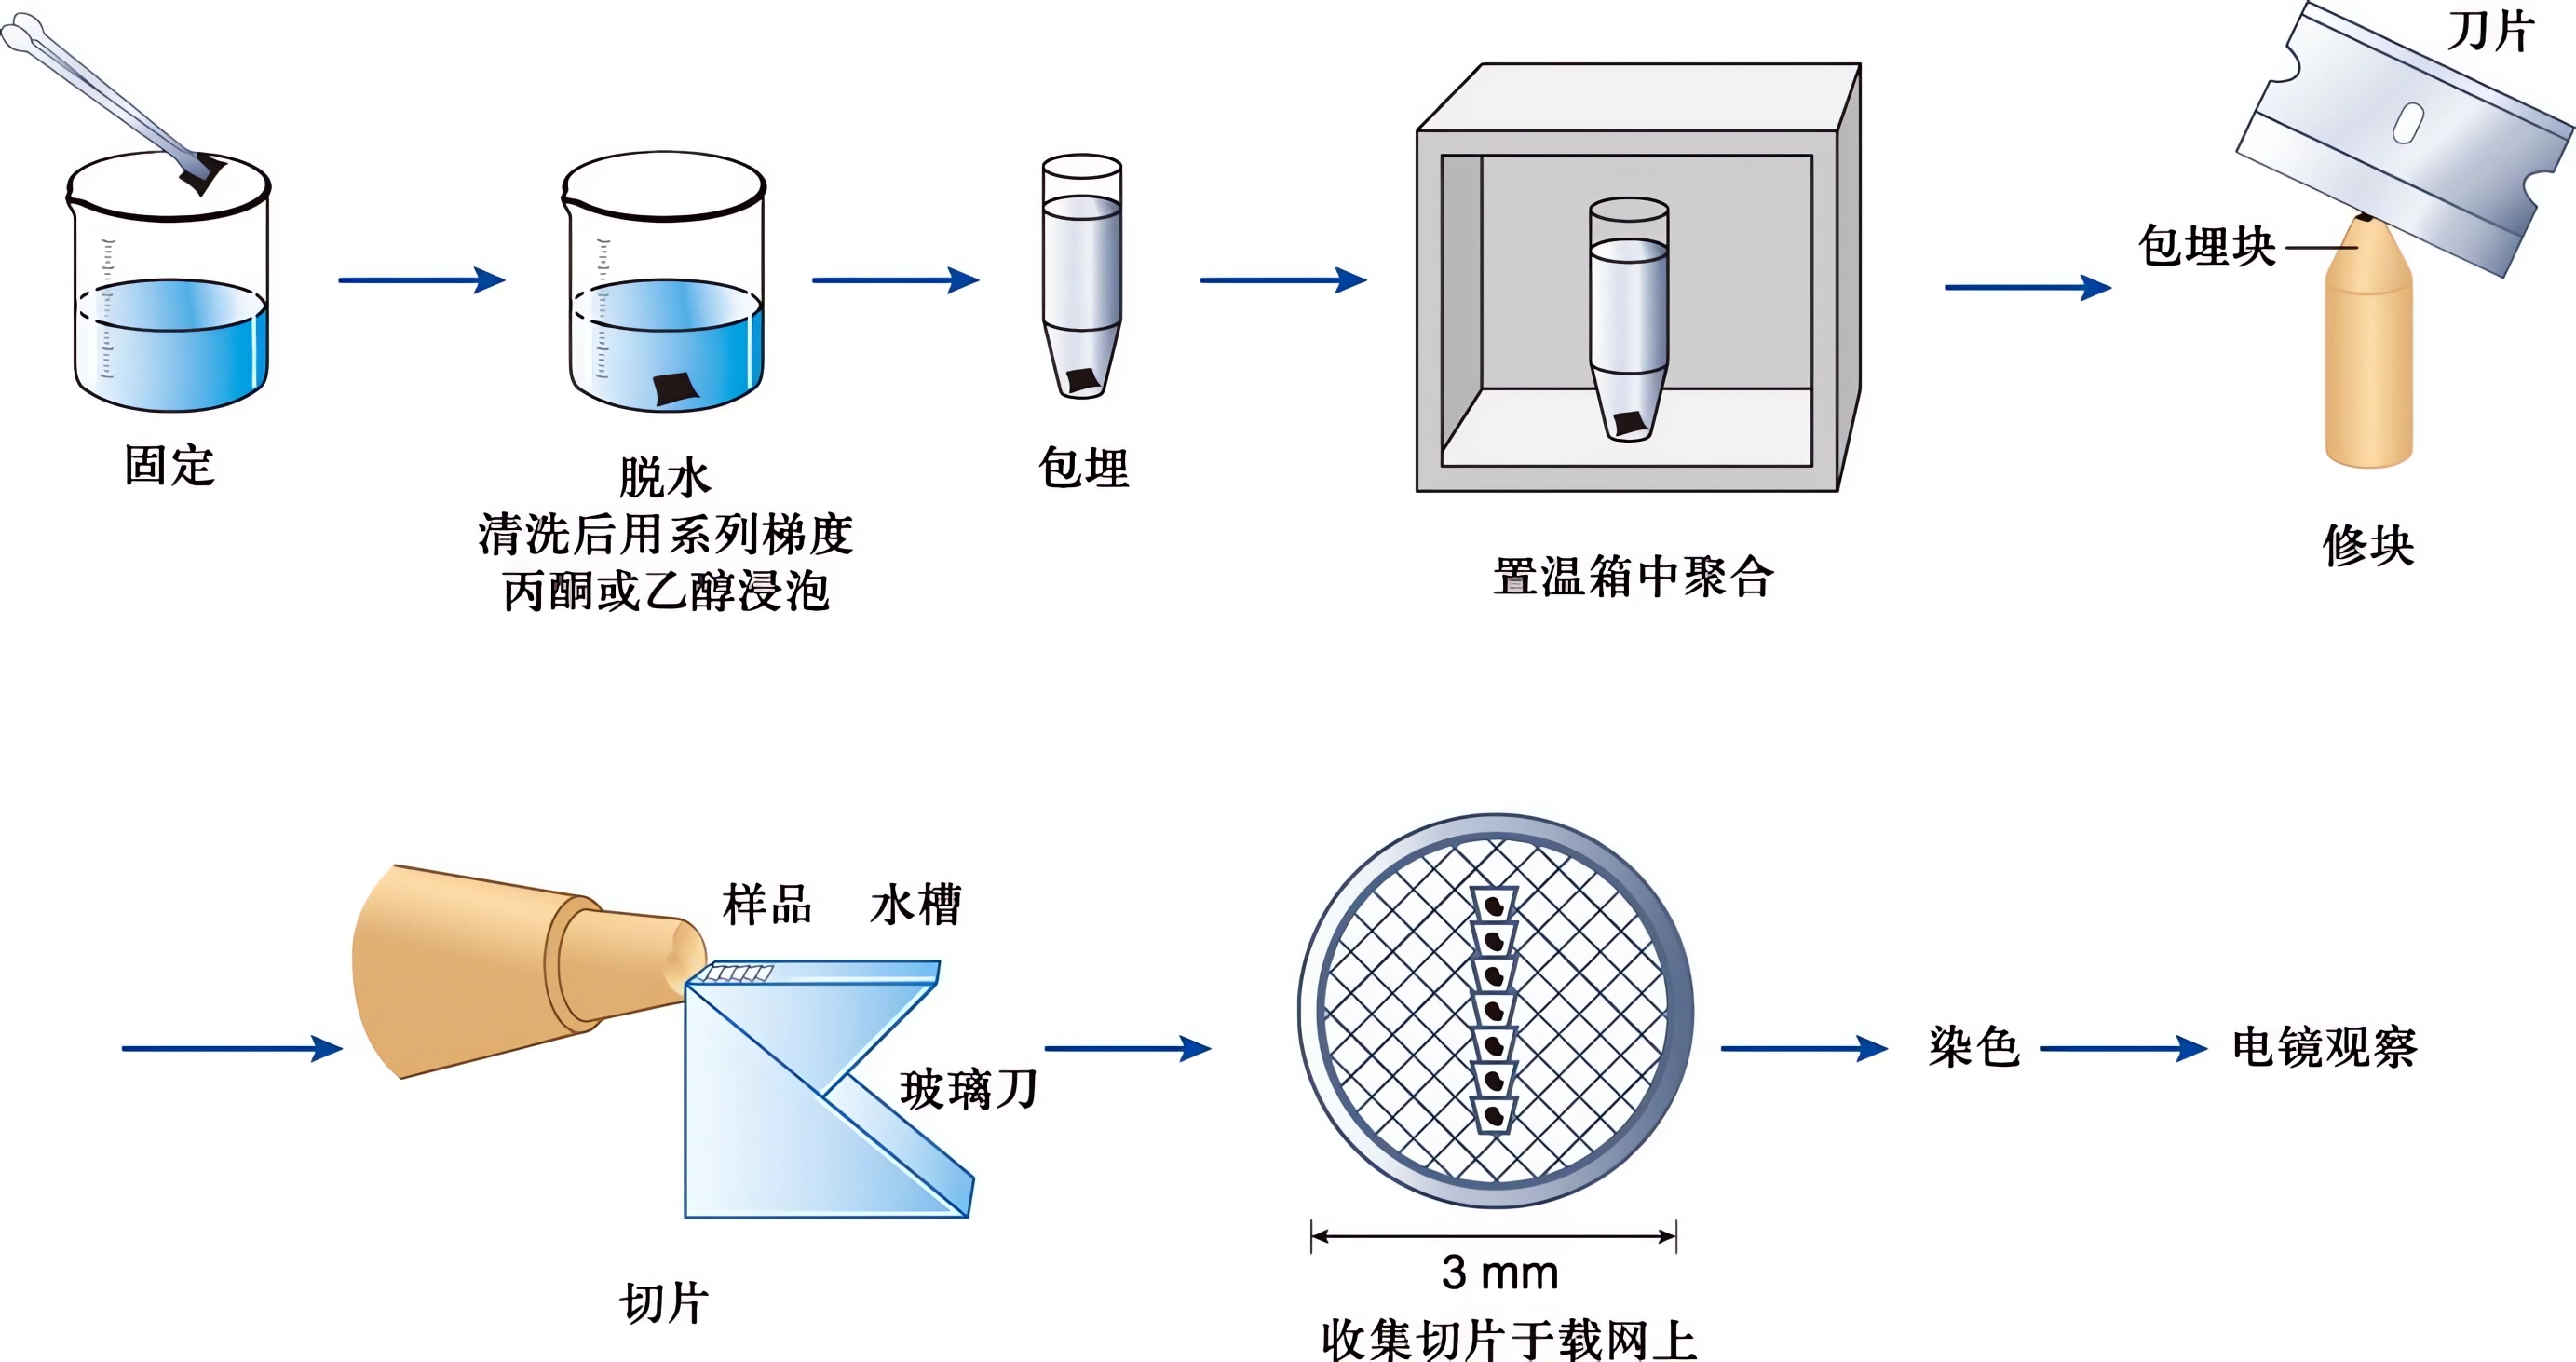
\includegraphics[width=\linewidth]{Pics/超薄切片流程}
	\caption{超薄切片流程}
	\label{fig:prcs_ultr_thn_sctn}
\end{figure}

\begin{description}
	\item[固定] 固定是保持样品真实性的最重要环节。这要求保持样品的形态和精细结构不发生改变,甚至是免疫原性不变。常用固定剂是戊二醛和锇酸(\ce{OsO4},四氧化锇)。还可额外使用冷冻等物理方法来保存细微结构。取样要快速,以防细胞结构溶解。
	\item[包埋] 包埋介质需要有良好的机械性能,以便切片。生物样品含水多,包埋剂却是疏水的,所以在包埋之前要进行脱水。常用包埋剂是各种环氧树脂。
	\item[切片] 切片常用玻璃刀或钻石刀。切片需捞在覆盖有支持膜(如Formvar膜)的载网(铜网或镍网)上。
	\item[染色] 用重金属盐染色。锇酸染脂质,柠檬酸铅染蛋白质、乙酸双氧铀染核酸。
\end{description}

应用超薄切片技术,几乎可以观察各种细胞的超微结构。

超薄切片技术还可与放射同位素自显影、细胞化学、免疫化学和原位杂交等技术结合,在超微结构水平上完成蛋白质与核酸等组分定性、定位和半定量研究。

\begin{figure}[htbp]
	\centering
	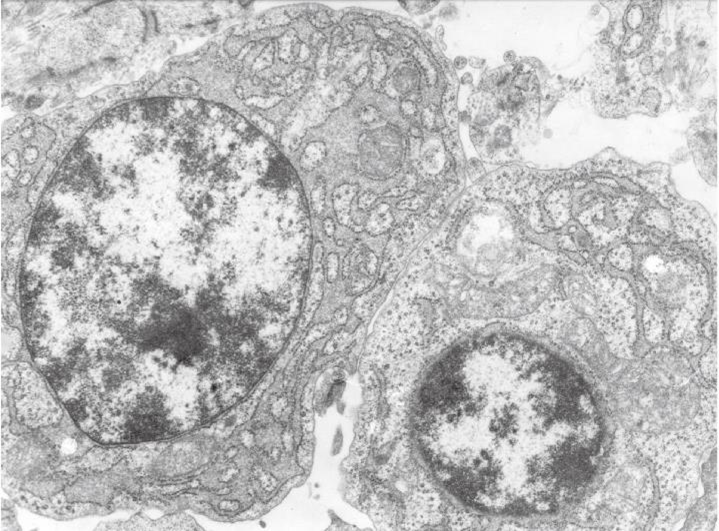
\includegraphics[width=0.5\linewidth]{Pics/超薄切片技术显示的动物细胞超微结构}
	\caption{超薄切片技术显示的动物细胞超微结构}
	\label{fig:ultrathinSectioningTechnologyShowingUltrastructureOfAnimalCells}
\end{figure}

\paragraph{负染色技术}

\begin{figure}[htbp]
	\centering
	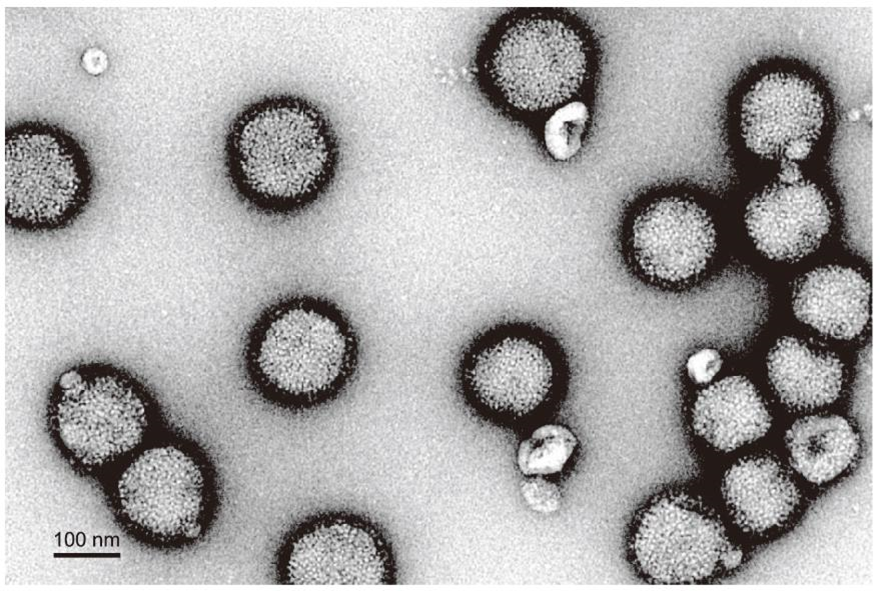
\includegraphics[width=0.5\linewidth]{Pics/流感病毒负染色电镜照片}
	\caption{流感病毒负染色电镜照片}
	\label{fig:influenzaVirusNegativeStainingElectronMicrograph}
\end{figure}


\paragraph{冷冻蚀刻技术}

\begin{figure}[htbp]
	\centering
	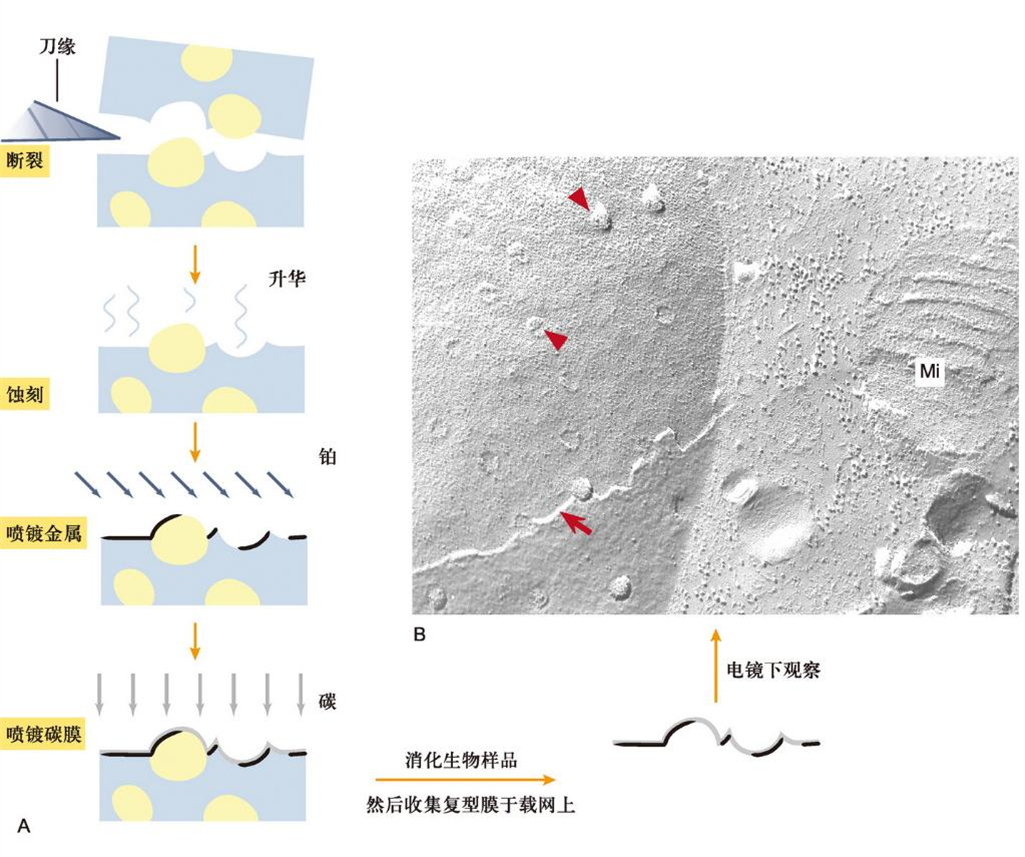
\includegraphics[width=\linewidth]{Pics/冷冻蚀刻技术示意图}
	\caption{冷冻蚀刻技术示意图}
	\label{fig:cryoFractureTechniqueSchematicDiagram}
\end{figure}

\subsection{扫描隧道显微镜(STM)}

特点:
\begin{itemize}
	\item 具有原子尺度的高分辨率;
	\item 可以在真空、大气、液体等多种环境测量;
	\item 非破坏性测量。
\end{itemize}

原子力显微镜


\section{核酸技术}

\subsection{核酸测序}

核酸测序测的是一级结构,即碱基排列顺序。

使核酸测序发生革命性变化的因素是:
\begin{itemize}
	\item 限制性内切酶(RE)的发现,能对DNA进行特异性切割;
	\item PAGE电泳技术的发展,能分辨单个核苷酸长度差异的序列。
\end{itemize}

下面介绍四代DNA测序技术。四代DNA测序技术的总结见\autoref{tab:DNA测序技术}。

\begin{table}[htbp]
	\centering
	\begin{tabularx}{\textwidth}{|c|C|c|c|c|c|c|}
		\hline
		代数 & 名称 & 准确性 & 读长 & 通量 & 扩增 & 合成 \\ \hline
		\multirow{2}{*}{第一代} & 双脱氧法(Sanger法) & \multirow{2}{*}{{\color{red}很高}} & \multirow{2}{*}{中} & \multirow{2}{*}{极低} & \multirow{5}{*}{是} & 是 \\ \cline{2-2} \cline{7-7}
		& 化学断裂法 &  &  &  &  & {\color{red}否} \\ \cline{1-5} \cline{7-7}
		\multirow{3}{*}{第二代} & 454焦磷酸 & \multirow{3}{*}{较高} & \multirow{3}{*}{短} & \multirow{3}{*}{极高} &  & \multirow{6}{*}{是} \\ \cline{2-2}
		& Illumina/Solexa &  &  &  &  &  \\ \cline{2-2}
		& SOLiD/Applied Biosystem &  &  &  &  &  \\ \cline{1-6}
		\multirow{2}{*}{第三代} & HeliScope & \multirow{4}{*}{高} & \multirow{4}{*}{长} & \multirow{2}{*}{中等} & \multirow{4}{*}{否} &  \\ \cline{2-2}
		& 单分子实时测序(PacBio SMRT) &  &  &  &  &  \\ \cline{1-2} \cline{5-5}
		\multirow{2}{*}{第四代} & 离子流 &  &  & \multirow{2}{*}{很高} &  &  \\ \cline{2-2} \cline{7-7}
		& 纳米孔(Oxford Nanopore) &  &  &  &  & {\color{red}否} \\ \hline
	\end{tabularx}
	\caption{DNA测序技术,“扩增”指需要大量样本,“合成”指边合成边测序}
	\label{tab:DNA测序技术}
\end{table}

\subsubsection{第一代测序}

\paragraph{双脱氧法}

双脱氧法也称末端终止法、Sanger法。它是最常用的第一代测序方法。具体原理见\autoref{fig:sanger_dna}。

\begin{figure}[p]
	\centering
	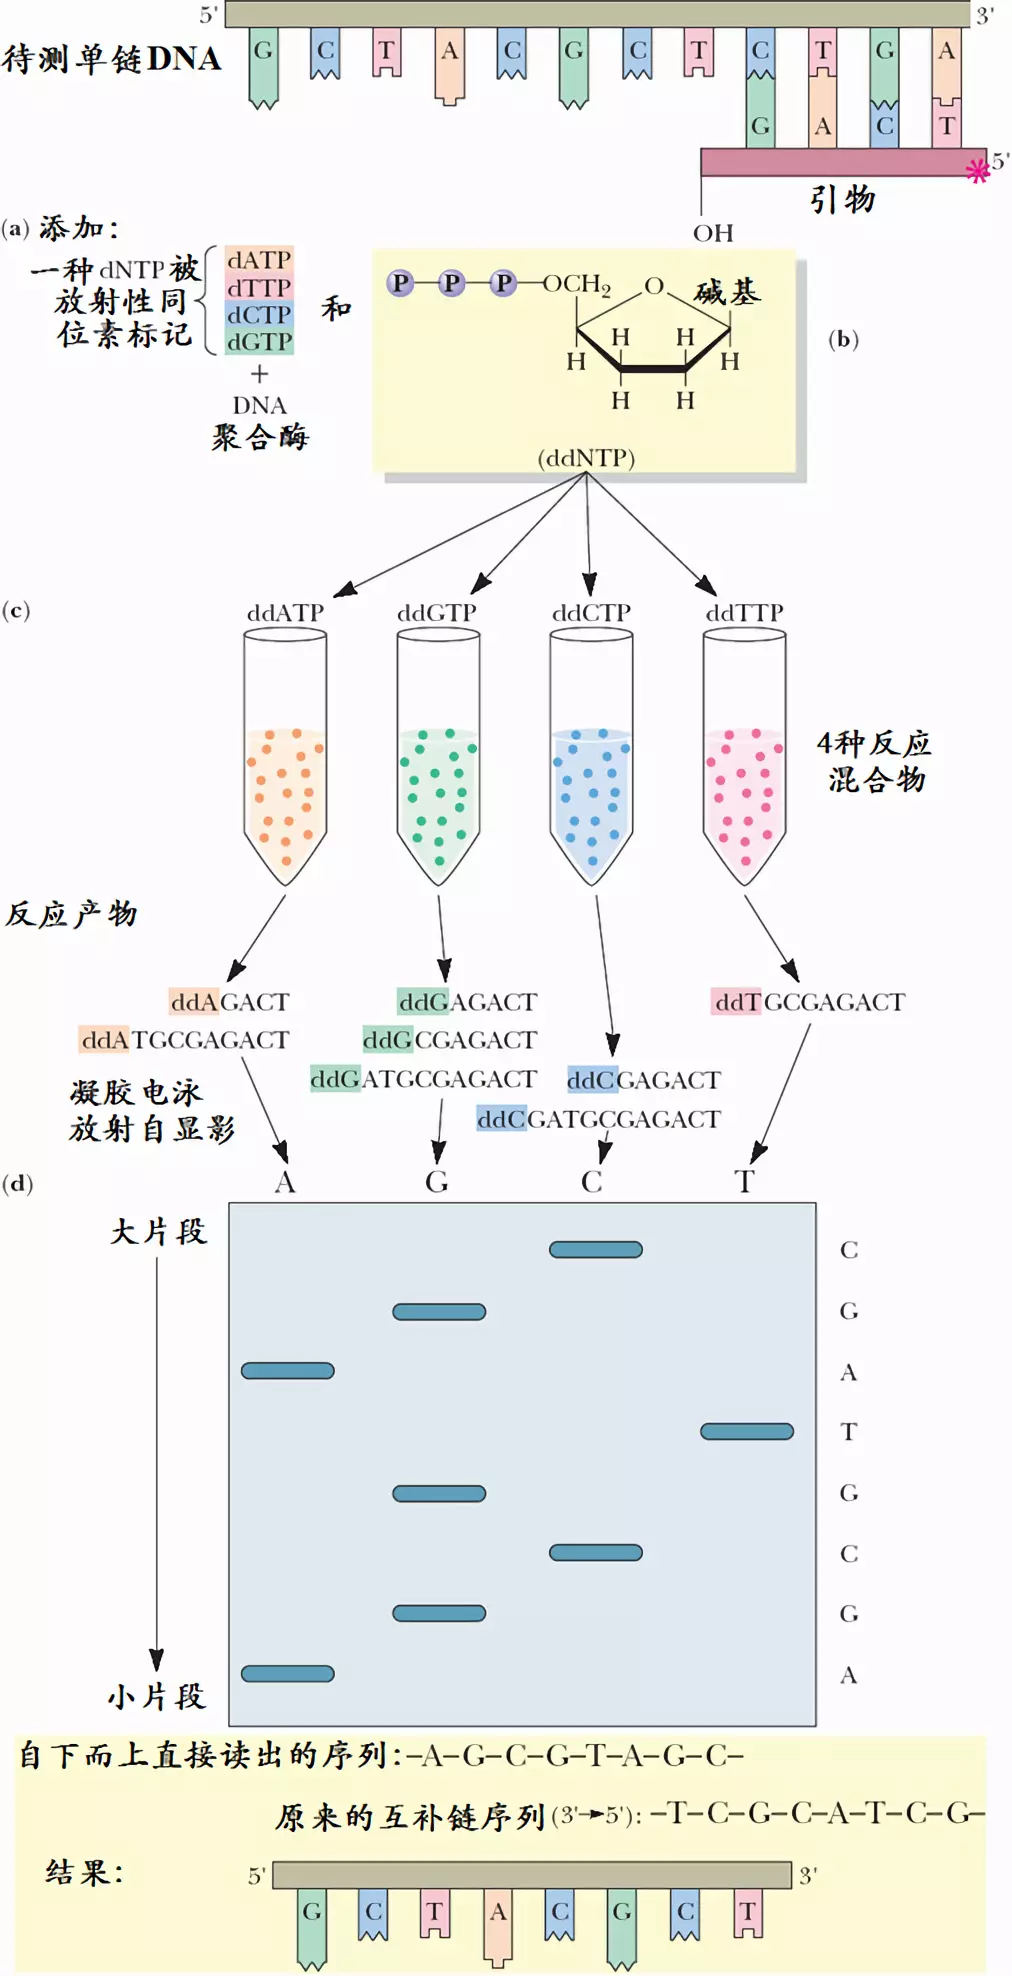
\includegraphics[width=0.7\linewidth]{Pics/Sanger法DNA测序}
	\caption{双脱氧法测序原理}
	\label{fig:sanger_dna}
\end{figure}

\paragraph{碱基特异性化学断裂法}

又称化学断裂法、Maxam-Gilbert法。

化学断裂法需要进行四组平行的反应:

\begin{description}
	\item[G特异性剪切] 在碱性条件下,先用硫酸二甲酯(DMS)处理,然后再使用哌啶处理;
	\item[嘌呤(A+G)碱基特异性剪切] DNA先进行酸处理,然后再加DMS;
	\item[嘧啶(C+T)碱基特异性剪切] 先用肼处理,然后用哌啶处理;
	\item[C特异性剪切] 在高盐下,先用肼处理,然后用哌啶处理;
\end{description}

进行聚丙烯酰胺凝胶电泳和放射自显影。比较G、A+G、C+T和C各个泳道,自下而上从自显影片上就可读出DNA序列。

\begin{figure}[htbp]
	\centering
	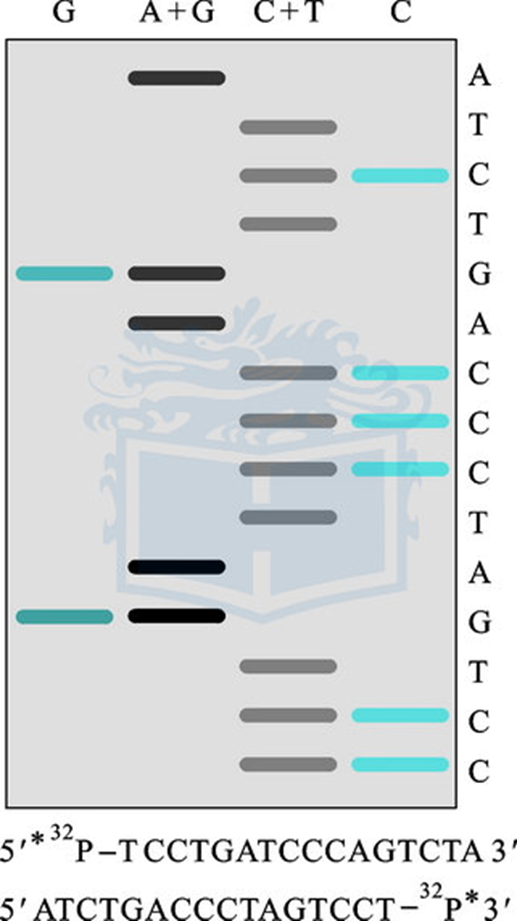
\includegraphics[width=0.3\linewidth]{Pics/化学断裂法测序}
	\caption{化学断裂法测序}
	\label{fig:MG_sequencing}
\end{figure}


\subsection{核酸分离纯化}

\subsubsection{酚-氯仿-异戊醇抽提}

细胞裂解后分离上清液,加入苯酚、氯仿、异戊醇(体积比$25:24:1$)。
\begin{itemize}
	\item 苯酚可竞争氢键,使蛋白质变性;
	\item 氯仿可以溶解苯酚等脂溶性物质,去除杂质;
	\item 异戊醇降低表面张力,消泡。
\end{itemize}

用乙醇和\ce{NaCl}沉淀DNA。
\begin{itemize}
	\item 加入\ce{Na+},可以中和DNA携带的负电荷。
\end{itemize}

75\%乙醇洗涤。

用TE buffer溶解DNA。

\subsubsection{质粒提取——SDS碱裂解法}

三个溶液:
\begin{description}
	\item[溶液I] 溶菌酶、\SI{50}{\mmol\per\L}葡萄糖、\SI{25}{\mmol\per\L} Tris pH 8.0,\SI{10}{\mmol\per\L}EDTA
	\begin{itemize}
		\item 溶菌酶溶解细胞壁;
		\item 葡萄糖维持溶液渗透压,防止DNA受机械剪切力损伤;
		\item EDTA可螯合金属离子,抑制DNase、促进溶菌酶的作用。
	\end{itemize}
	\item[溶液II] \SI{0.2}{\mmol\per\L} \ce{NaOH}、1\% SDS
	\begin{itemize}
		\item \ce{NaOH}调pH为碱性,使DNA变性;
		\item SDS使蛋白质变性。
	\end{itemize}
	\item[溶液III] \SI{50}{\mmol\per\L}醋酸钠、大量冰醋酸
	\begin{itemize}
		\item 形成缓冲体系,调pH至中性。
	\end{itemize}
\end{description}

后续使用酚仿抽提提取。

\subsubsection{RNA提取}


\subsubsection{核酸纯度检测}

使用Nanodrop分光光度计检测:
\begin{description}
	\item[A260/A230] \SI{230}{\nm}处是糖类、胍盐等杂质的吸收峰。纯净的核酸样品该值约为2.5。
	\item[A260/A280] 前者是核酸的吸收峰,后者是蛋白质的吸收峰,反映核酸被蛋白质污染的程度。纯净双链DNA约为1.8,RNA大于2。这一参数是最重要的。
\end{description}

浓度换算关系:1OD相当于\SI{50}{\ug\per\ml}的dsDNA、\SI{37}{\ug\per\ml}的ssDNA、\SI{40}{\ug\per\ml}的RNA。

\subsection{核酸电泳}

\subsubsection{基本原理}

电泳是带电颗粒在电场作用下发生定向迁移的过程。

电场中分子的迁移速率取决于分子的带电性、分子量、空间结构等。

\subsubsection{琼脂糖凝胶电泳}

\paragraph{琼脂糖凝胶的制备}

加入溴化乙锭(EB)、SYBR Green等结合DNA的试剂,便于检测。

\subsection{核酸杂交}

\subsubsection{DNA杂交——Southern Blot}


\subsubsection{RNA杂交——Western Blot}

\subsubsection{膜上印迹杂交}

\subsubsection{基因芯片}

\subsection{基因工程}

\subsubsection{分子克隆}

\subsubsection{聚合酶链式反应(PCR)}

\paragraph{PCR的反应体系}

\begin{description}
	\item[DNA模板]
	\item[DNA引物]
	\item[DNA pol]
	\item[dNTP]
	\item[\ce{Mg^{2+}}] 这是DNA聚合酶所必须的。有时加入的是\ce{Mn^{2+}}进行易错PCR,因为DNA聚合酶的校对活性依赖于\ce{Mg^{2+}}。
\end{description}

\paragraph{PCR操作流程}

预变性




\section{蛋白质技术}

\subsection{蛋白质分离纯化}

\subsection{蛋白质定量}

\subsubsection{凯氏定氮法}

蛋白质与硫酸和催化剂共热,硫酸铵与NaOH释放氨气,可测定含氮量/0.16

\subsubsection{双缩脲法}

碱性溶液中 cuso4 540nm比色 标准曲线

灵敏度较差,样品用量大。

\subsubsection{Lowry法}

福林酚显色  福林酚不是酚

660nm比色

\subsubsection{BCA法}

562nm BCA还原二价铜离子。溶液中不能含有EDTA或dtt等还原剂

\subsubsection{Bradford法}

考马斯亮蓝G-250在酸性溶液中鲜红色,与碱性氨基酸结合后蓝色。595nm

与还原剂兼容,但受去垢剂影响较大。

\subsubsection{工具——分光光度仪}

朗伯比尔光吸收定律 $A=\epsilon bc$

\subsection{蛋白质电泳}

\subsubsection{电泳准备}

竖着、

缓冲液:25mM Tris-HCl  190nMGLY
浓缩胶:偏中性,把蛋白质拉到同一条线上
分离胶:偏碱性


